\documentclass[fleqn]{article}
\usepackage[english]{babel}
\usepackage{amsmath}
\usepackage{amsthm}
\usepackage{graphicx}
\usepackage[utf8]{inputenc}

%%%%%%%% MARGIN
\usepackage[left=1in, right=1in, top=0.8in, bottom=0.8in]{geometry}

%%%%%%%% NO PARAGRAPH INDENT
% https://tex.stackexchange.com/questions/27802/set-noindent-for-entire-file
\setlength\parindent{0pt}

%%%%%%%% SUB-FIGURE PACKAGE
\usepackage{subcaption}

\usepackage{pdfpages}

%%%%%%%% HYPERREF PACKAGE
\usepackage{hyperref}
\hypersetup{linkcolor=blue}
\hypersetup{citecolor=blue}
\hypersetup{urlcolor=blue}
\hypersetup{colorlinks=true}

%%%%%%%% MULTI-COLUMNS PACKAGE
\usepackage{multicol}

%%%%%%%% SETS DEFINITIONS
\usepackage{amssymb}
%%%% Important sets
\renewcommand{\O}{\mathbb{O}}
\newcommand{\N}{\mathbb{N}}
\newcommand{\Z}{{\mathbb{Z}}}
\newcommand{\Q}{{\mathbb{Q}}}
\newcommand{\RR}{{\mathbb{R}}}

%%%% Statistics
\newcommand{\E}[1]{\mathbb{E}\left[#1 \right]}
\newcommand{\V}[1]{\mathbb{V}\left[#1 \right]}
\newcommand{\cov}[1]{\mathrm{Cov}\left[#1 \right]}

%%% Misc Math
% Spaces after/before left/right
\let\originalleft\left
\let\originalright\right
\renewcommand{\left}{\mathopen{}\mathclose\bgroup\originalleft}
\renewcommand{\right}{\aftergroup\egroup\originalright}

% Norm and abs
\newcommand{\norm}[1]{\left\lVert#1\right\rVert}
\newcommand{\abs}[1]{\left\lvert#1\right\rvert}

%%%% Superscript to the left
% https://latex.org/forum/viewtopic.php?t=455
\usepackage{tensor}
\newcommand{\app}[3]{\tensor*[^{#1}]{\left(#2, #3\right)}{}}


%%%%%%%% SPLIT EQUATIONS
% https://tex.stackexchange.com/questions/51682/is-it-possible-to-pagebreak-aligned-equations
\allowdisplaybreaks

%%%%%%%% CODE RENDERING
% Compile with flag -shell-escape
\usepackage{minted}

%%%%%%%% EXAM PACKAGE
\usepackage{mathexam}

%%%%%%%% CHANGE MARGINS ITEMIZE
\usepackage{enumitem}

%%%%%%%% START DOCUMENT

\ExamClass{EC0301 - Time Series}
\ExamName{Assignment \#5}
\ExamHead{\today}

\let\ds\displaystyle

\begin{document}
 \vspace{0.3cm}
   % Information of the student
   \begin{itemize}[leftmargin=6.25cm, labelsep=0.5cm]

     \item[\textit{Name}] \scalebox{1.2}{David Plazas Escudero} % Name
     \item[\textit{Student code}] 201710005101 % Code

   \end{itemize}
\vspace{0.3cm}

% Each of the items to solve
\begin{enumerate}
\item \textit{Make a program that estimates an ARMA(1,1) model using the conditional and non-conditional algorithms studied in class. Estimate an ARMA(1,1) model for the data from last assignment and compare the obtained results with an estimation already implemented in your programming language (statistical module).}

The code to estimate an ARMA(1,1) model is presented below. Note that the model takes a parameter \texttt{method} if the derivative in the estimation process is calculated numerically or analytically (see the comment). Additionally, takes a boolean parameter \texttt{cond} to apply the conditional or non-conditional estimation procedure.
\begin{minted}{python}
import numpy as np


# method -> 1 : Uses numerical approximation of derivative.
#        -> 2 : Uses exact derivative (iterative calculation).
# cond   -> 0 : Uses non-conditional estimation.
#        -> 1 : Uses conditional estimation.
def fit_ARMA11(xs, beta0, tol=1e-7, h=1e-7, method=1, cond=True):
    def estimate_epsilon(xs, beta):
        e = np.zeros((xs.size, 1))
        for t in range(1, xs.size):
            e[t] = xs[t] - beta[0]*xs[t-1] + beta[1]*e[t-1]
        return e

    def exact_derivative(xs, e, beta):
        d = np.zeros((xs.size, 1))
        for t in range(1, xs.size):
            d[t] = beta[1]*d[t-1] + e[t-1]
        return d

    def estimate_epsilon_noncond(xs, beta, n_iter=100, tol=1e-7):
        etas = [xs[-1]]
        T = xs.size
        for T0 in range(T-1, 0, -1):
            etas.append(xs[T0] - beta[0, 0]*xs[T0-1] + beta[1, 0]*etas[-1])

        ws = [beta[0, 0]*xs[0] - beta[1, 0]*etas[-1]]
        k = 0
        while k <= n_iter:
            ws.append(beta[0, 0]*ws[-1])
            if ws[-1] <= tol:
                break

        xs_ext = np.hstack((np.array(ws), xs))
        e = estimate_epsilon(xs_ext, beta)
        return e[-(T+1):], ws[0]

    if cond:
        T = xs.size - 1
    else:
        T = xs.size
    beta = np.array(beta0).reshape(2, 1)
    Z = np.zeros((T, 2))
    k = 0
    norms = []
    while True:
        if cond:
            ek = estimate_epsilon(xs, beta)
            Z[:, 0] = xs[:-1]
            xs0 = xs
        else:
            ek, w0 = estimate_epsilon_noncond(xs, beta)
            xs0 = np.hstack((w0, xs))
            Z[:, 0] = xs0[:-1]
        if method == 1:
            aux = np.array([[0], [h]])
            ekh = estimate_epsilon(xs0, beta + aux)
            Z[:, 1] = -((beta[1] + h)*ekh[:-1, 0] - beta[1]*ek[:-1, 0])/h
        elif method == 2:
            derivative = exact_derivative(xs0, ek, beta)
            Z[:, 1] = -derivative[1:, 0]
        estimated_diff = np.linalg.inv(Z.T.dot(Z)).dot(Z.T).dot(ek[1:])
        new_beta = beta + estimated_diff
        norms.append(np.linalg.norm(beta - new_beta, ord=np.Inf))
        if norms[-1] < tol:
            break
        beta = new_beta
        k += 1
    return new_beta, norms
\end{minted}

The model was tested using an artificial ARMA(1,1) simulation with $x_0=0$, $\beta=(0.3, -0.5)^T$ and $T=1000$. The code for this simulation is presented below.
\begin{minted}{python}
import matplotlib.pyplot as plt
import scipy.stats as st

plt.rc('text', usetex=True)
plt.rcParams.update({'font.size': 16})


def simulateARMA11(x0, T, beta, sigma2=1):
    xs = np.zeros(T+1)
    xs[0] = x0
    ts = np.linspace(0, T+1, T+1)
    e = st.norm.rvs(size=xs.shape, scale=sigma2)
    for t in range(1, T+1):
        xs[t] = beta[0]*xs[t-1] + e[t] - beta[1]*e[t-1]
    return ts, xs
    

# Test for ARMA(1,1) - beta = [[0.3], [-0.5]]
# Conditional
ts, xs = simulateARMA11(0, 1000, [0.3, -0.5])
beta_cond, norms_cond = fit_ARMA11(xs, [0.5, -0.3], method=2, cond=True)
print('beta_cond', beta_cond[0], beta_cond[1])

# Non-conditional
beta, norms = fit_ARMA11(xs, [0.5, -0.3], method=2, cond=False)
print('beta', beta[0], beta[1])
plt.plot(norms, 'k')
plt.xlabel('$k$')
plt.ylabel('$||\\beta^{k+1}-\\beta^k||_\infty$')
plt.savefig('test.pdf', bbox_inches='tight')
plt.clf()
\end{minted}

Setting $\beta^0=(0.5, -0.3)^T$, the estimated beta obtained using the conditional estimation and the analytical calculation for the derivative was $\hat{\beta}=(0.32009,-0.49825)^T$ and the non-conditional with the analytical was $\hat{\beta}=(0.32010, -0.49820)^T$, which are both close to the real $\beta$. In Figure \ref{fig:exp}, the convergence of the norm can be observed, only for the latter experiment.
\begin{figure}[H]
    \centering
    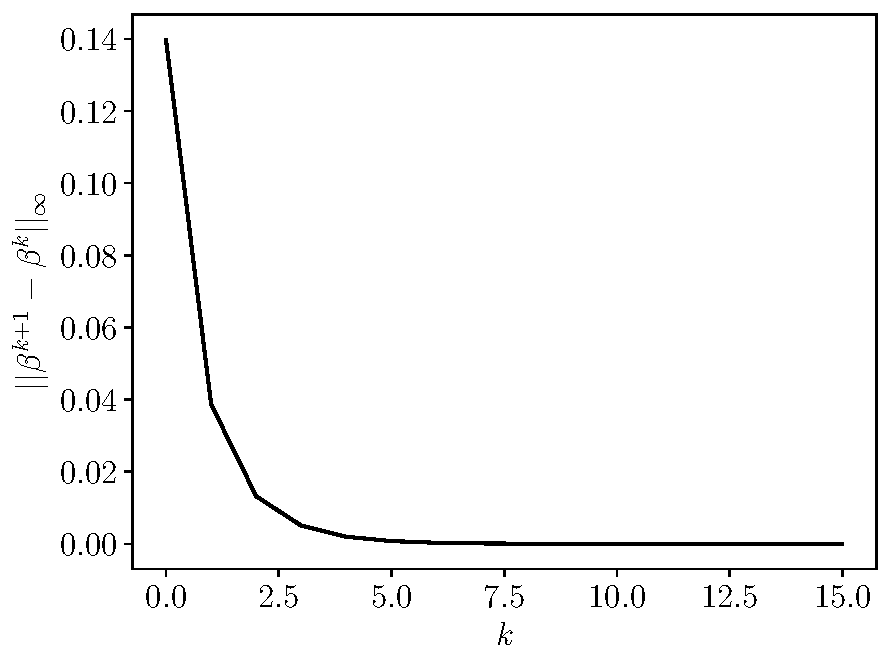
\includegraphics[scale=0.5]{figs/test.pdf}
    \caption{Norm convergence for ARMA experiment.}
    \label{fig:exp}
\end{figure}

Now, for the data from last assignment, the code to fit the model using the implemented code and Statsmodels' fit method is presented:
\begin{minted}{python}
import statsmodels.tsa.arima.model as sm

# Read data
file = open('seguimiento5.csv', 'r')
file = file.read().split('\n')[1:-1]
data = np.array([line.split(',')[1] for line in file], dtype=float)

# Estimate ARMA(1,1)
beta, norms = fit_ARMA11(data[:100], [0.4, -0.2], method=1, cond=True)
plt.plot(norms, 'k')
plt.xlabel('$k$')
plt.ylabel('$||\\beta^{k+1}-\\beta^k||_\infty$')
plt.savefig('test.pdf', bbox_inches='tight')
plt.clf()
print('My beta', beta[0], beta[1])
mod = sm.ARIMA(data, order=(1, 0, 1))
res = mod.fit()
print('Statsmodels beta', res.arparams, -res.maparams)
print(res.summary())
\end{minted}
\newpage
It is important to mention that the only the first 101 points were considered for the implemented function, due to numerical stability reasons and convergence. For the Statsmodels' fit, the whole time series was used. Setting $\beta^0=(0.4, -0.2)^T$ with the non-conditional algorithm with the analytic calculation of the derivative, $\hat{\beta}=(0.45590,-0.52430)^T$, whereas the Statsmodels' estimation was $\hat{\beta}=(0.50197, -0.47589)^T$. This shows that both approximations where close. Finally, in Figure \ref{fig:data}, the norm convergence in this experiment is presented.
\begin{figure}[H]
    \centering
    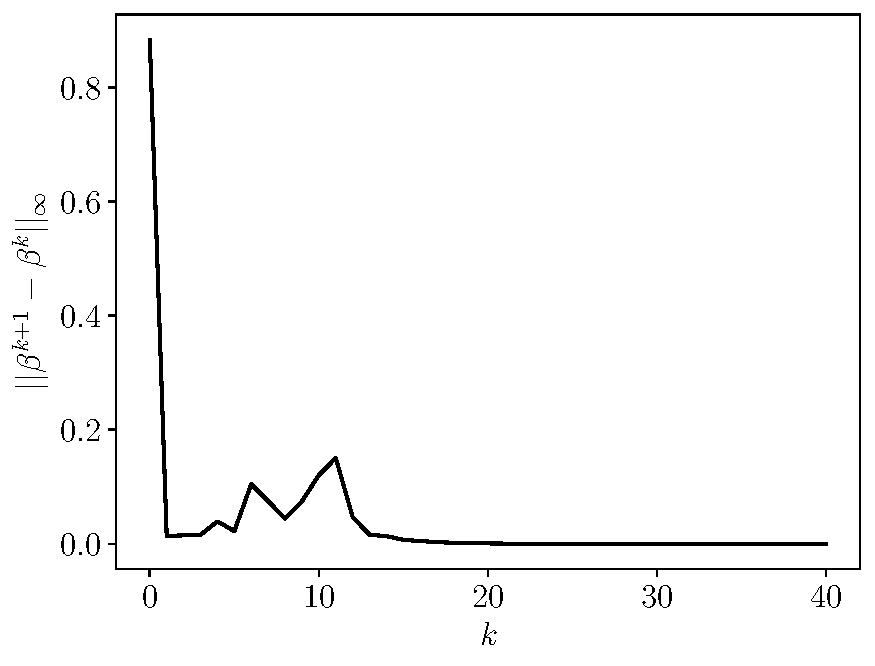
\includegraphics[scale=0.5]{figs/data.pdf}
    \caption{Norm convergence for last assigment's data experiment.}
    \label{fig:data}
\end{figure}

\end{enumerate}
\end{document}
